% 2.3.2.CmakeMethod.tex
%	Last update: 2020/02/32 F.Kanehori
%newpage
\subsubsection{CMakeを使用した場合}
\label{subsubsec:CmakeMethod}
\parindent=0pt

Cmakeはout of source (out of place)によるビルドに対応しています。
これはソースツリーの外側にビルドツリーを生成する機能で、次のような特徴があります。
\Vskip{-.5\baselineskip}
\begin{itemize}
  \item	互いに干渉しない複数のビルドツリーを作成することができる。
  \item	ビルドツリーが削除されてもソースツリーに影響が及ばない。
\end{itemize}
\Vskip{-.5\baselineskip}
我々はCMakeをout of sourceの方法で使用します。

\medskip
ソースツリーおよびビルドツリーは、ライブラリおよびアプリケーションのそれぞれで
次のようになるでしょう
(図\ref{fig:SpringheadLibraryTree}および図\ref{fig:ApplicationTree})。

\Vskip{-.2\baselineskip}
\begin{narrow}
    \begin{figure}[h]
	\begin{center}
	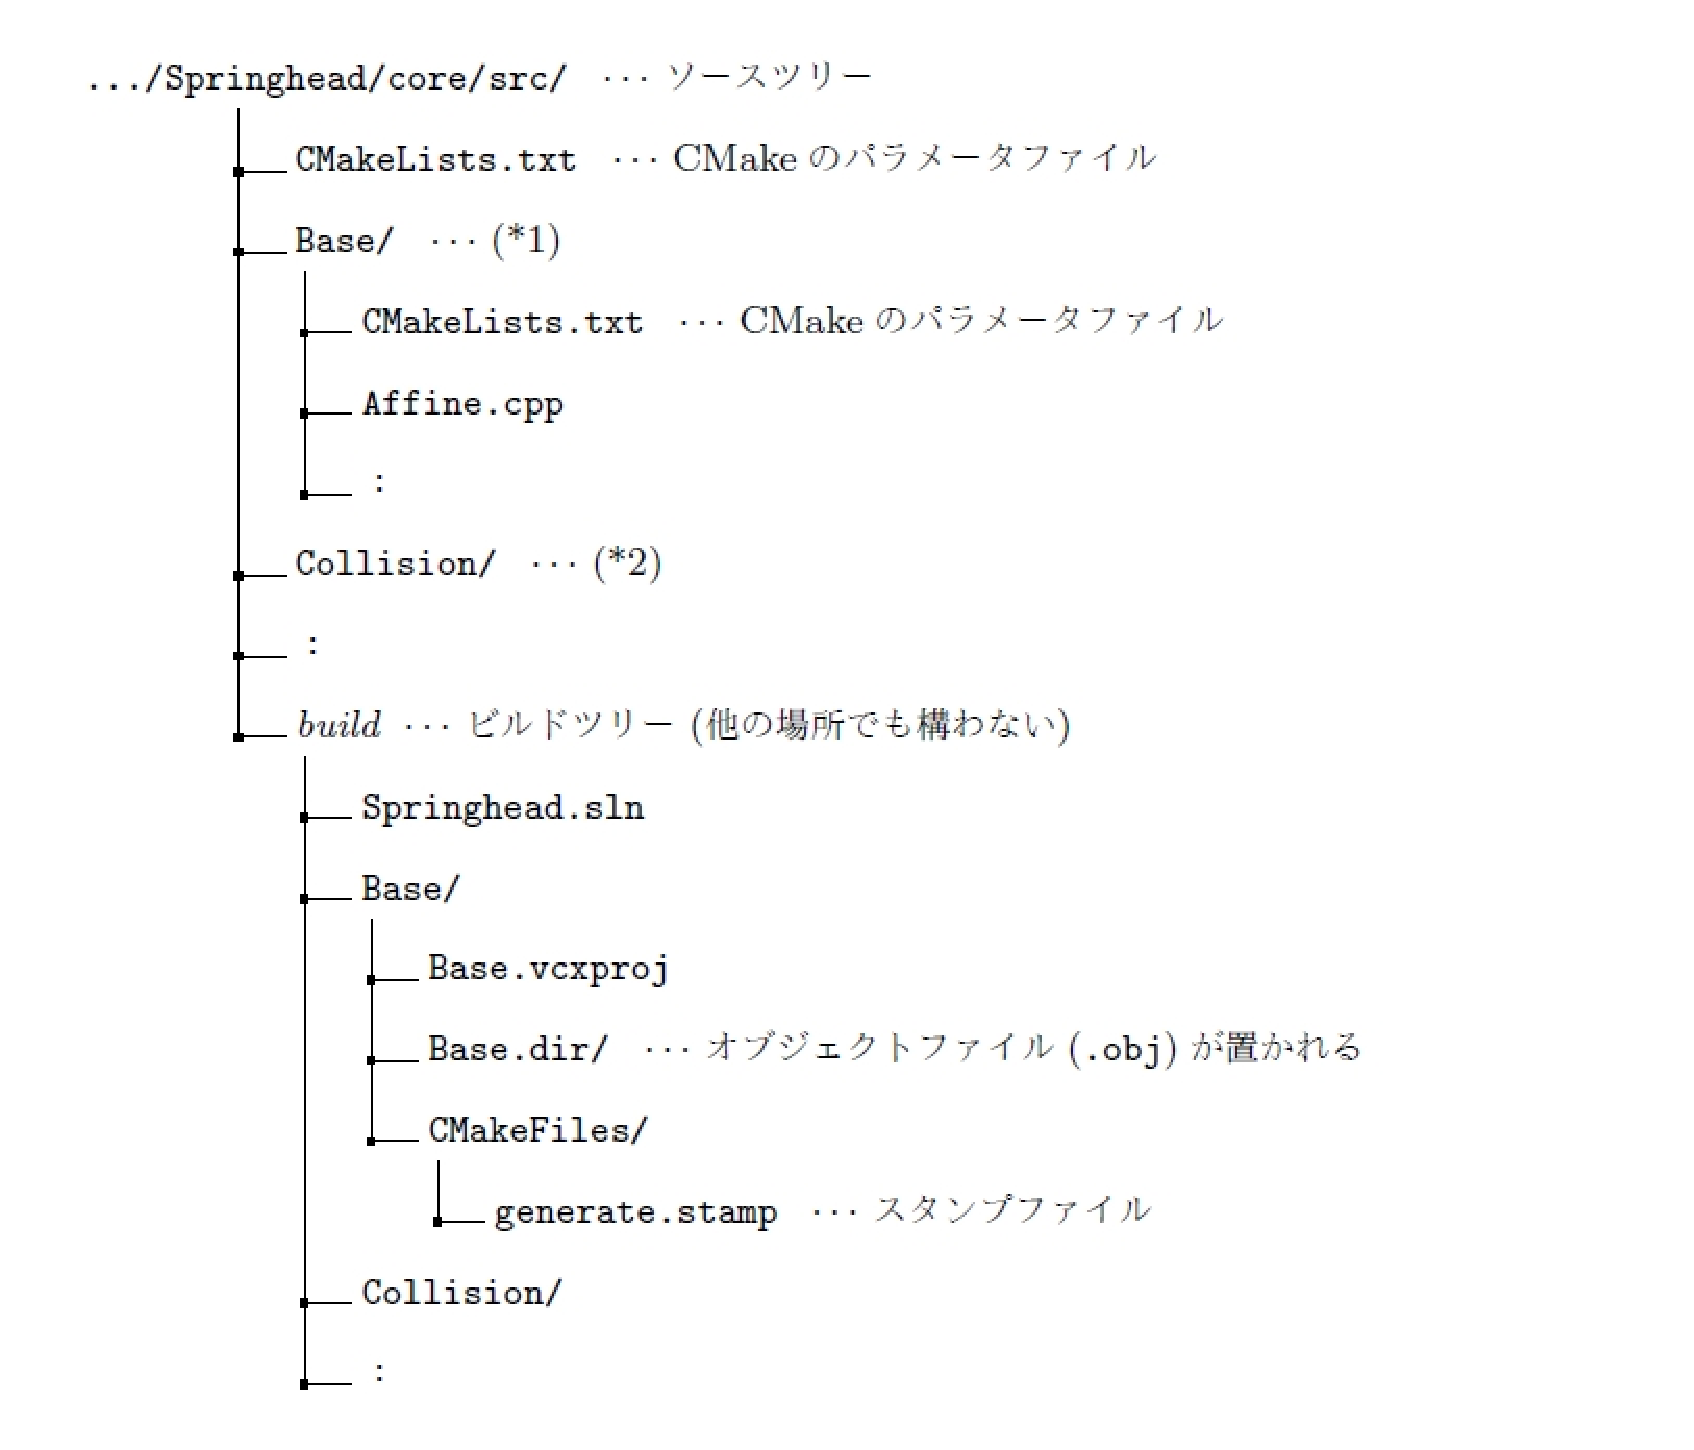
\includegraphics[width=.9\textwidth]{fig/LibraryTree.eps}
	\end{center}
	\caption{Springhead Library構成}
	\label{fig:SpringheadLibraryTree}
    \end{figure}
\end{narrow}
%\begin{narrow}\begin{figure}[h]
%    \begin{narrow}[40pt]\begin{minipage}{\textwidth}
%	{\footnotesize{\dirtree{%
%		.1 \hspace{-10mm}C:/Springhead/core/src/ \Anno{ソースツリー}.
%		.2 CMakeLists.txt \Anno{ライブラリ全体のCMakeのパラメータファイル}.
%		.2 Base/ \Anno{(1)}.
%		.3 CMakeLists.txt \Anno{プロジェクトBaseのCMakeのパラメータファイル}.
%		.3 :.
%		.2 Collision/ \Anno{(2)}.
%		.2 :.
%		.2 \BldDir \Anno{ビルドツリー (他の場所でも構わない)}.
%		.3 Springhead.sln \Anno{生成されたソリューションファイル}.
%		.3 Base/.
%		.4 Base.vcxproj \Anno{生成されたプロジェクトファイル}.
%		.4 Base.dir/ \Anno{オブジェクトファイル(\tt{.obj})が置かれる}.
%		.4 CMakeFiles/.
%		.5 generate.stamp \Anno{スタンプファイル}.
%		.3 Collision/.
%		.3 :.
%	}}}
%	\medskip
%    \end{minipage}\end{narrow}
%    \caption{Springhead Library構成}
%    \label{fig:SpringheadLibraryTree}
%\end{figure}\end{narrow}

\Vskip{-.2\baselineskip}
\begin{narrow}
    \begin{figure}[h]
	\begin{center}
	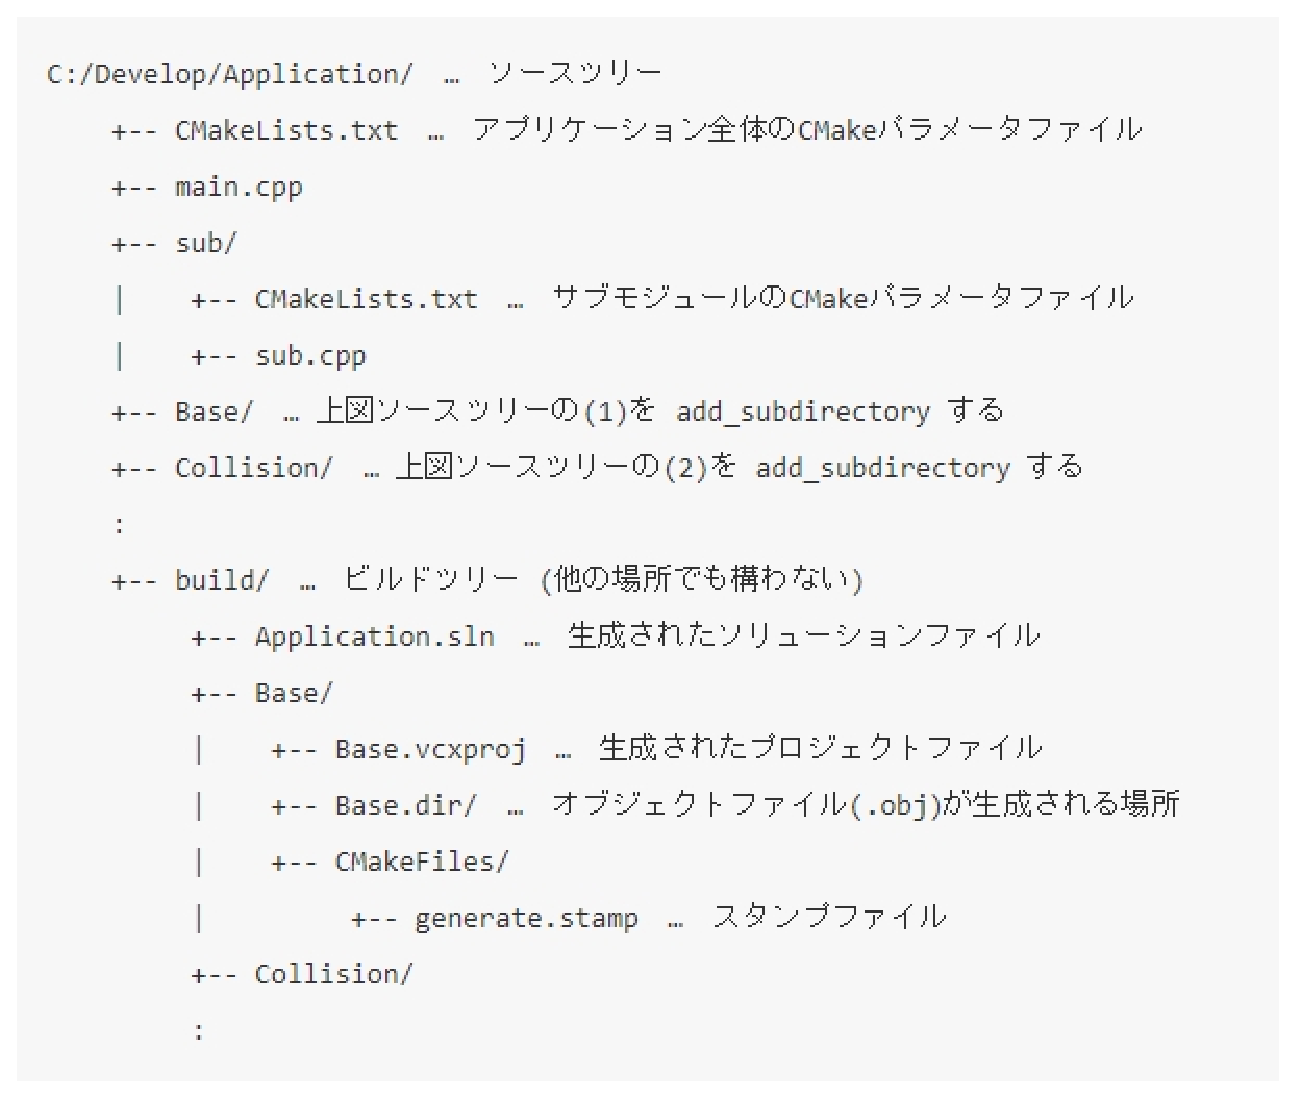
\includegraphics[width=.9\textwidth]{fig/ApplicationTree.eps}
	\end{center}
	\caption{Application構成}
	\label{fig:ApplicationTree}
    \end{figure}
\end{narrow}
%\begin{narrow}\begin{figure}[h]
%    \begin{narrow}[40pt]\begin{minipage}{\textwidth}
%	{\footnotesize{\dirtree{%
%		.1 \hspace{-10mm}C:/Develop/Application/ \Anno{ソースツリー}.
%		.2 CMakeLists.txt \Anno{アプリケーション全体のCMakeのパラメータファイル}.
%		.2 main.cpp.
%		.2 Sub/.
%		.3 CMakeLists.txt \Anno{サブモジュールのCMakeのパラメータファイル}.
%		.3 sub.cpp.
%		.2 Base/ \Anno{上図ソースツリーの(1)を\tt{add\_subdirectoryする}}.
%		.2 Collision/ \Anno{Spsringheadの(*2)を指すようにする}.
%		.2 :.
%		.2 \BldDir \Anno{ビルドツリー (他の場所でも構わない)}.
%		.3 Application.sln \Anno{生成されたソリューションファイル}.
%		.3 Base/.
%		.4 Base.vcxproj \Anno{生成されたプロジェクトファイル}.
%		.4 Base.dir/ \Anno{オブジェクトファイル(\tt{.obj})が生成される場所}.
%		.4 CMakeFiles/.
%		.5 generate.stamp \Anno{スタンプファイル}.
%		.3 Collision/.
%		.3 :.
%	}}}
%	\medskip
%    \end{minipage}\end{narrow}
%    \caption{Application構成}
%    \label{fig:ApplicationTree}
%\end{figure}\end{narrow}

\medskip
ライブラリをビルドしたときもアプリケーションをビルドしたときも、
それぞれのビルドにおける生成物は、
すべてそれぞれのビルドツリー内におかれることに注意してください。
言い換えると、 ライブラリのオブジェクトファイルが、
複数のビルドツリーに独立して配置されるということです。

% end: 2.3.2.CmakeMethod.tex
